\textsf{Cassis} est un simulateur de caches sur architecture multi-c\oe ur développé dans le cadre d'un PFA -- Projet au Fil de l'Année -- à l'\textsc{Enseirb-Matmeca}, sur une idée proposée par Denis BARTHOU pour le compte de l'\textsf{INRIA}. L'\textsf{INRIA} est un institut publique de recherche français en informatique et automatismes ; et bien que ce projet soit réalisé dans un cadre scolaire, l'objectif est de le rendre utilisable par les équipes de recherche des thématiques associées aux caches et au parallèlisme.

\section{Cadre du simulateur}

\paragraph{}
Un simulateur est un programme qui va reproduire le fonctionnement d'un système afin de pouvoir en étudier certaines caractéristiques de manière moins contraignante que sur le système réel. Dans le cas du programme \textsf{Cassis}, c'est l'utilisation des caches par un programme donné qui est simulée.

\subsection{Origine du projet}

\paragraph{}
La mémoire est de nos jours l'un des principaux facteurs de ralentissement des programmes. Une mauvaise gestion de la mémoire peut être désastreuse au niveau des performances, et pourtant, il n'existe pas de moyen efficace et précis de connaître l'utilisation de la mémoire au niveau des caches. Le but de \textsf{Cassis} est donc d'étudier l'utilisation précise des caches par un programme, afin d'aider l'utilisateur à tester les performances du programme, ainsi que les analyser pour les améliorer.

\paragraph{}
Le besoin d'un tel simulateur est avant tout dû au manque d'informations sur les caches. Deux phénomènes se produisent du côté des constructeurs de processeurs. D'une part ils doivent les optimiser afin d'être concurrents, et il devient alors difficile pour eux de rajouter des fonctionnalités dédiées aux développeurs afin d'améliorer leur code, par exemple des compteurs exacts du nombre de \emph{hits}. D'autre part il n'est pas dans leur intérêt de révéler le fonctionnement de leurs produits, pour des raisons économiques évidentes. Par exemple, le \emph{prefetching} permet de charger des lignes de caches en avance en fonction des accès mémoires courants du programme et cette fonctionnalité n'est pas implémentée dans le simulateur car son fonctionnement n'est pas totalement divulgué.

\paragraph{}
L'intérêt d'un tel simulateur est donc de pouvoir tester des programmes en produisant certaines statistiques, mais aussi de pouvoir tester l'exécution sur des architectures qui n'existent pas afin de connaître la pertinence d'une nouvelle politique de cohérence par exemple. Seuls les caches de données sont simulés, le but étant d'essayer d'optimiser la mémoire d'un programme. Le chargement du code du programme est fait par le processeur sans intervention de l'utilisateur.

\subsection{Outils à disposition de l'utilisateur}

Le simulateur s'appuie sur des outils préexistants, pour la génération des traces et de l'architecture. Les outils listés ci-dessous sont ceux utilisés par l'équipe de projet. Si d'autres outils offrent des fonctionnalités similaires, ils peuvent être utilisés en remplacement tant que les fichiers d'entrée du programme sont dans le bon format.

\paragraph{HWLOC} est un logiciel qui permet de récupérer l'architecture des caches d'une machine. Il permet de générer un fichier xml que nous enrichissons. La paramétrisation de l'architecture des caches ne prend pas en compte les caches d'instructions, mais seulement les caches de données. L'utilisation de ce fichier est détaillé dans la section \ref{param_xml}.

\paragraph{MAQAO} (Modular Assembly Quality Analyzer and Optimizer) est un outil d'analyse et d'optimisation de programmes. Une seule fonctionnalité de \textsf{MAQAO} est utilisée, celle qui permet d'instrumenter un programme binaire afin de récupérer les instructions réalisées pendant l'exécution. Le paramétrage de \textsf{MAQAO} est effectué grâce à un fichier lua pour générer des traces de la forme voulue.

\paragraph{}
L'utilisateur peut aussi vouloir comparer les résultats de la simulation. Bien qu'il n'existe par actuellement de tel simulateur pour faire la comparaison, il existe des compteurs hardware -- par exemple \textsf{PAPI} -- qui permettent de connaître certaines statistiques sur les caches. Les limites du simulateur seront donc étudiées, afin de valider son bon fonctionnement par rapport au comportement attendu.

\section{Déroulement de la simulation}

\paragraph{}
La simulation consiste à rejouer un certain nombre d'instructions, et de comptabiliser certaines métriques à destination de l'utilisateur. Comme il s'agit d'une simulation, tout ne se passe pas exactement comme dans le cas réel. Il est donc nécessaire d'expliciter les similitudes comme les différences afin que l'utilisateur ne soit pas surpris à la fois par les résultats, et à la fois par les méthodes de calculs si son objectif est de modifier le code.

\paragraph{}
Dans le cadre de la simulation, seules les références aux données sont stockées en mémoire, c'est-à-dire l'ensemble des étiquettes qui permettent d'identifier les différentes données. Pour une ligne de cache de taille $64$ octets par exemple, seule la première case est réellement stockée en mémoire, les $56$ autres octets correspondant aux données sont inutiles pour réaliser les statistiques.

\subsection{Traitement d'une instruction : load/store}

\paragraph{}
La simulation, même d'un programme parallèle, est une séquence d'instructions effectuant des modifications (lecture ou écriture) sur les caches. Les deux premières possibilités pour une instruction sont, soit une lecture de donnée, soit une écriture. Une fois le type d'instruction connu, il faut la faire correspondre au c{\oe}ur sur lequel elle a été effectuée. Si la donnée est déjà présente dans le cache de plus bas niveau (L1), alors il s'agit d'un \emph{Hit}. Sinon, il faut rechercher la donnée dans la hiérarchie. A noter que pour des raisons d'efficacité, la simulation ajoute la donnée au moment même où l'on traite le cache: on prévoit qu'elle sera bientôt fournie par un cache de niveau supérieur en cas de \emph{Miss}.

\paragraph{}
L'idée de l'algorithme est donc la suivante: on applique l'instruction courante au L1 correspondant, et si la donnée n'est pas présente, on remonte au niveau d'au dessus. Les protocoles de cohérence étant relatifs à un niveau donné, ils sont appliqués dès que possible afin d'éviter d'avoir à monter puis à redescendre dans la hiérarchie pour des questions de complexité. Cette idée de prévision permet généralement de gagner du temps mais posent certains problèmes qui seront explicités.

\paragraph{}
Un algorithme pour le traitement général d'une instruction est le suivant: 
\begin{enumerate}
  \item{il s'agit d'un \emph{load} ou d'un \emph{store}}
  \item{la donnée est présente dans le cache ou non
      \begin{enumerate}
      \item{si non, l'ajouter et faire :}
      \item{appel de la procédure de suppression en cas de cache plein}
      \item{mettre à jour les états de cohérence des différents caches du niveau concernés par la même donnée}
      \item{chercher la donnée dans la hiérarchie}
      \item{revenir au point 2 s'il faut chercher la donnée dans un cache de plus haut niveau}
  \end{enumerate}}
  \item{mettre à jour les statistiques de remplacement sachant qu'une ligne a été accédée}
  \item{dans le cas d'un \emph{store}, propager l'action de modification dans tous les caches de niveaux supérieurs}
\end{enumerate}

\paragraph{}
Dans le code du simulateur, le traitement d'une instruction différe dans le cas d'un \emph{load} ou d'un \emph{store}. En effet les deux versions se distinguent par la dernière étape, où dans le cas d'un \emph{store}, les caches parents doivent être prévenus de la modification même en cas de \emph{Hit}. Si par exemple, en cas de \emph{Hit} lors d'un \emph{store} d'une donnée A dans un L1, le L2 doit être informé afin de pouvoir invalider la même donnée dans les autres L2. Cependant, si la lecture du programme apparaît comme une vraie modification des données (comme pour la politique \emph{Write-Through}), les statistiques sont bien réalisées de manière à suivre le cas du \emph{Write-Back}, où une modification dans un cache de bas niveau provoque une réécriture dans les caches de plus haut niveau le plus tard possible afin de limiter le coût de ces échanges entre les caches.

\paragraph{}
Le paragraphe précédent pose quelque uns des problèmes issus de la manière prédictive de voir les choses. Les problèmes fondamentaux sont la recherche d'une donnée dans la hiérarchie, l'ajout d'une ligne dans un cache, et la conservation des propriétés des caches inclusifs et exclusifs.

\subsection{Rapatriement prédictif d'une ligne}

\paragraph{}
Le fait de supposer qu'il est possible d'ajouter une donnée avant même de l'avoir trouvé dans la hiérarchie ne change rien au niveau des statistiques produites, mais impose de prendre soin à certaines étapes du traitement d'une instruction. En cas de \emph{Miss}, trois traitements peuvent être réalisés, selon l'architecture fournie en entrée du programme. Une première solution consiste à rechercher les données par snooping, c'est-à-dire parmis les caches du même niveau partageant le même parent. Cette étape doit être réalisée avant la mise à jour des états de cohérence. Par exemple en cas de \emph{store} sur une donnée avec la politique de cohérence MESI, les autres caches vont devoir invalider leur copie locale de la même donnée pour garantir la cohérence. D'où l'obligation de réaliser le protocole de snooping avant d'éventuelles invalidations.

\paragraph{}
Une seconde solution consiste à utiliser un \emph{directory manager}, afin de rechercher les données dans les caches en dessous (impossible pour un L1). Dans l'implémentation choisie, le traitement par directory manager implique de réellement parcourir l'ensemble des caches ayant pour parent le cache courant. Dans le cas réel, une table comportant la partie étiquette des lignes de caches est tenue à jour grâce à un \emph{directory manager}. Cependant, vu la complexité des messages à envoyer pour garantir la consistance de la table, le choix du parcours de tous les caches a été réalisé.

\paragraph{}
Si la donnée n'a pas été trouvée via le \emph{snooping} ou grâce à un \emph{directory manager}, une demander est effectuée au cache de plus haut niveau qui effectue une autre recherche jusqu'à éventuellement joindre la mémoire principale.

\paragraph{}
La particularité du rapatriement prédictif des données est à prendre en compte dans l'écriture des politiques de cohérences. En effet certaines politiques se basent sur la présence ou non de la même ligne dans le niveau du cache demandant la donnée, voir à ce sujet les conditions de transitions d'automates dans la partie \ref{aut}. Il faut alors être conscient que la donnée est déjà dans le niveau lorsque les voisins sont prévenus.

\subsection{Problème d'ajout de ligne dans un cache plein}

\paragraph{}
L'ajout d'une donnée dans un cache est également un problème compliqué. Il faut commencer par identifier dans quel block la donnée va se retrouver, puis demander à la politique de remplacement un emplacement dans ce block pour mettre la nouvelle donnée. Si le block n'était pas plein, l'ajout d'une ligne dans un cache se résume à trouver le block et ajouter la donnée.

\paragraph{}
Cependant, si le cache est plein, une ligne à evincer est choisie. Il faut ensuite rapatrier cette ligne dans le cache de niveau supérieur, si elle n'y était pas déjà présente et faire un \emph{Write-Back} si la ligne supprimée avait été modifiée. Si la donnée n'était pas présente dans le cache de niveau supérieur, il faut l'y ajouter. Une subtilité relative au traitement prédictif de la recherche d'une donnée est à prendre en compte. En effet, si un L1 ajoute une donnée $A$ et qu'il doit pour cela supprimer la donnée $B$, il va falloir ajouter cette donnée dans le L2 correspondant. Or si ce L2 est plein, il peut évincer la donnée $A$. Le traitement étant prédictif, ce n'est pas la situation qui se produirait dans la réalité. Pour palier à ce problème, une donnée à ne surtout pas supprimer à été ajoutée en paramètre des fonctions relatives au replacement.


\subsection{Gestion des différents types de cache}
\paragraph{}
\textsf{Cassis} permet de gérer différents types de caches: inclusif, exclusif, non-inclusif orienté inclusif et non-inclusif orienté exclusif. Si la gestion des caches non-inclusifs est assez souple (on ne connaît pas précisément les choix faits par les constructeurs), la gestion des caches inclusifs et exclusifs s'attache à assurer que le type des caches est bien respecté.

\paragraph{}
Pour un cache inclusif, le cas problématique est la suppression d'une donnée. Il faut en effet assurer que les caches de plus bas niveau ayant pour père le cache inclusif ne conservent pas la donnée. La solution mise en {\oe}uvre consiste à invalider dans toute la hiérarchie en dessous de ce cache. Une gestion plus subtile est possible par une utilisation des \emph{directory manager}. Avant de supprimer une donnée, les caches en dessous sont consultés afin de connaître les données qu'ils possèdent. De cette manière, des priorités sont calculées pour la suppression des données, afin d'éviter d'avoir à invalider d'autres caches.

\paragraph{}
Ce problème est crucial au sens où il est très fréquemment rencontré. En effet, les politiques de remplacement peuvent être différentes entre les niveaux et dans une certaines mesures incohérentes. Si un cache L2 possède un remplacement de type FIFO alors que les L1 associés ont un remplacement de type LRU, les flags de remplacement vont faire que le L2 aura tendance à vouloir supprimer des données qui peuvent avoir été récemment utilisées dans les L1.

\paragraph{}
invalider hit exclusif

\section{Données simulées : analyses des statistiques}

Différentes statistiques sont relevées par le simulateur, les principales sont les \emph{misses}, les \emph{hits} et les \emph{write-backs}. Dans l'exemple ci dessous, on peut observer une sortie standard de \textsf{Cassis}: \\

\begin{lstlisting}
L3  basics   (misses:   6, hits:   0, writes_back:   0)
L2  basics   (misses:   6, hits:   0, writes_back:   0)
L1  basics   (misses:   4, hits:  44, writes_back:   1)
L1  basics   (misses:   6, hits:  42, writes_back:   2)
L2  basics   (misses:   0, hits:   0, writes_back:   0)
L1  basics   (misses:   0, hits:   0, writes_back:   0)
L1  basics   (misses:   0, hits:   0, writes_back:   0)
\end{lstlisting}


Il est également possible d'avoir plus de statistiques, voici le schéma maximal pour un seul cache:
\begin{lstlisting}
L1  basics     (misses:      8, hits:        40, writes_back:   4)
    evinctions (coherence:   4, capacity:    0, cache_types:    0)
    misses     (snooping:    3, above:       5, below:          0)
    broadcasts (coherence:   10, snooping:   8)
\end{lstlisting}


Ces statistiques ont été choisies afin que l'utilisateur puisse constater certains problèmes particuliers. Par exemple, un nombre trop élevé de \emph{write-backs} et/ou de \emph{coherence evinctions} révèle que les c\oe urs modifient les mêmes données et que la manière de paralléliser le code n'est donc pas efficace. \\

L'affichage des statistiques est configurable en ligne de commande, avec l'option \texttt{-v i}, pour $i$ allant de $1$ à $4$, selon le nombre de lignes de statistiques à afficher. La première ligne correpsond aux statistiques de base, qui ont déjà été vues. \\

Par rapport aux évictions de données, $3$ cas se présentent:
\begin{itemize}
\item coherence: ce cas se produit lorsqu'une donnée est invalidée dans un cache à cause d'une écriture dans un autre cache,
\item capacity: c'est le cas ``classique `` d'éviction: la taille du cache est trop faible pour contenir beaucoup de données,
\item cache\char`_types: ce cas se produit lorsqu'un cache exclusif donne une donnée: il doit l'invalider pour garantir l'exclusivité; ou encore lorsqu'un cache inclusif invalide une donnée: il doit également l'invalider dans les niveaux en dessous afin de conserver le caractère inclusif. \\ 
\end{itemize}

En cas de \emph{Miss}, $3$ solutions sont possibles pour trouver les données dans la hiérarchie:
\begin{itemize}
\item snooping: la donnée est obtenue via du snooping avec un cache de même niveau,
\item above: la donnée est obtenue en remontant dans la hiérarchie,
\item below: la donnée est obtenu en parcourant la hiérarchie vers les niveaux inférieurs. Dans le cas étudié, cette situation ne peut se présenter qu'avec l'utilisation de \emph{directory manager}. \\
\end{itemize}

Pour finir, $2$ types de \emph{broadcast} font partie des statistiques:
\begin{itemize}
\item coherence: cette statistique permet de comptabiliser les échanges de messages nécessaires aux politiques de cohérence, pour que les lignes des caches soient dans les bons états,
\item snooping: quand un cache fait une demande pour récupérer une donnée via le snooping. \\
\end{itemize}


Mais les statistiques ne sont pas les seuls paramètres d'analyse, la sélection des données à analyser à aussi un rôle important. Le simulateur permet de suivre les statistiques d'une ou plusieurs instructions données, et ainsi de déterminer quelles instructions causent des ralentissements à l'exécution, i.e. un trop grand nombre de \emph{misses}.

\subsection{\'Etapes de validation}
\begin{frame}
  \begin{block}{Pr\'esentation}
    \begin{itemize}
      \item Tests unitaires
      \item Validation durant le programme
      \item Comparaison avec des outils existants
      \item Benchmarks
    \end{itemize}
  \end{block}
  \begin{block}{Premiers outils de v\'erification}
    \begin{itemize}
      \item Validation des politiques basiques
      \item Validation du comportement inclusif
      \item Utilisation de \textsf{PAPI}
    \end{itemize}
  \end{block}
\end{frame}

\begin{frame}{Benchmarks basiques}
\begin{figure}[H]
   \begin{minipage}[l]{.46\textwidth}
     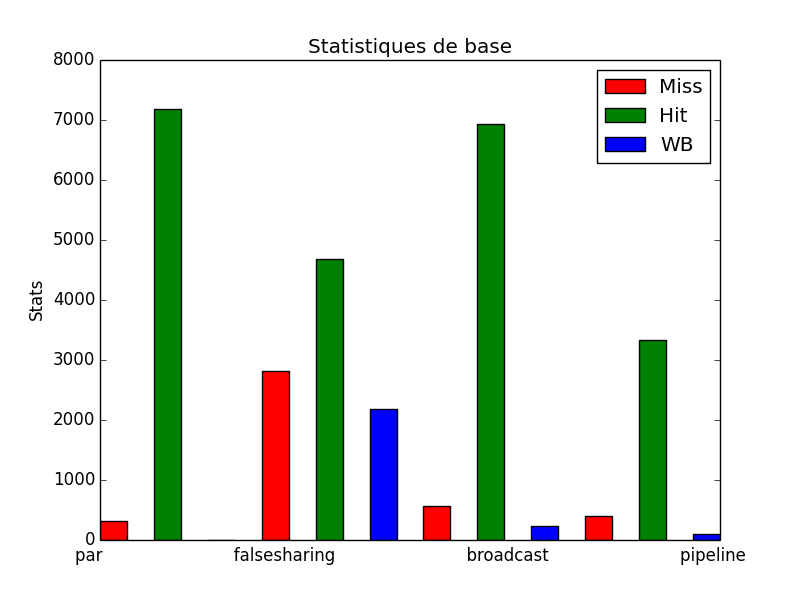
\includegraphics[scale=0.22]{images/stats_L1.png}
   \end{minipage} \hfill
   \begin{minipage}[r]{.46\textwidth}
     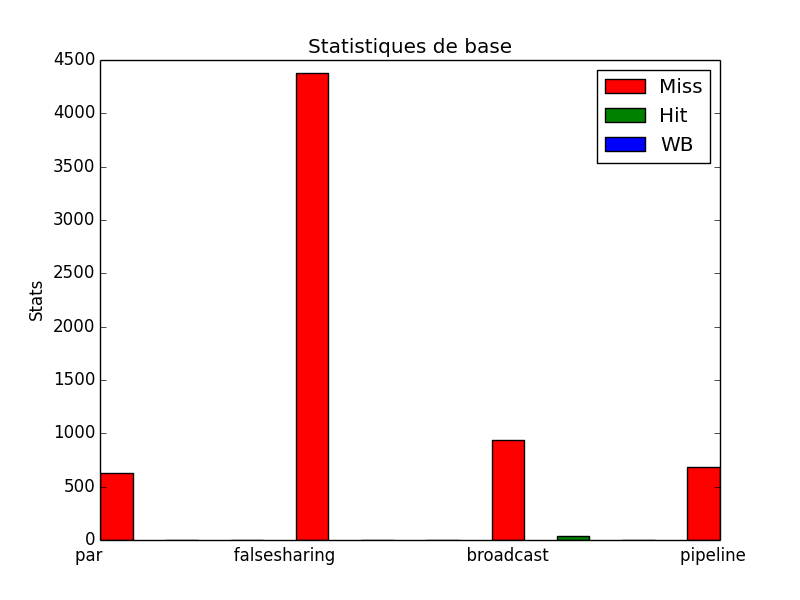
\includegraphics[scale=0.22]{images/stats_L2.png}
   \end{minipage}
\end{figure}

\begin{figure}[t!]
  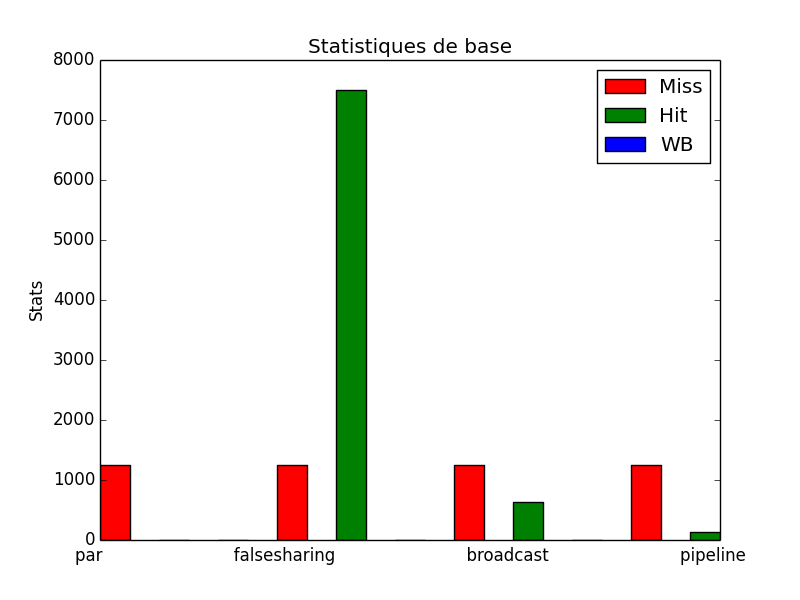
\includegraphics[scale=0.22]{images/stats_L3.png}
\end{figure}
\end{frame}

\begin{frame}{Benchmarks avanc\'es}
\begin{figure}[H]
   \begin{minipage}[l]{.46\textwidth}
     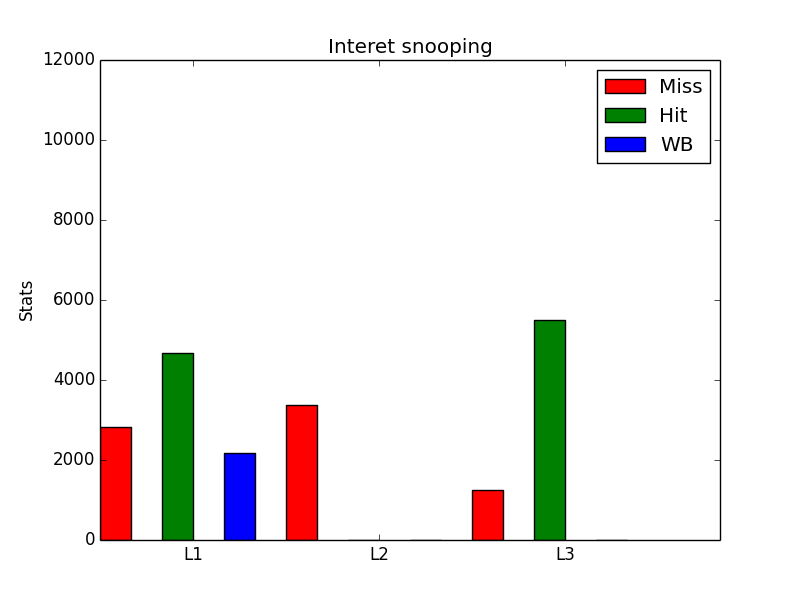
\includegraphics[scale=0.22]{images/stats_falsesharing_snooping.png}
   \end{minipage} \hfill
   \begin{minipage}[r]{.46\textwidth}
     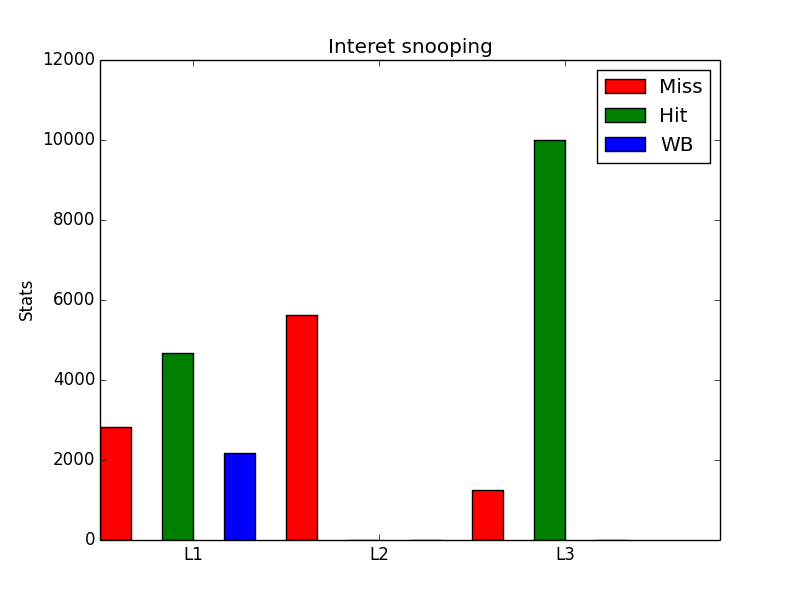
\includegraphics[scale=0.22]{images/stats_falsesharing_no_snooping.png}
   \end{minipage}
\end{figure}
  \begin{block}{Autres benchmarks}
    \begin{itemize}
      \item \emph{Directory manager}
      \item Politiques de coh\'erence MSI vs MESI
      \item Scalabilit\'e
    \end{itemize}
  \end{block}
\end{frame}

\subsection{Limites \`a  propos de la simulation des caches}
\begin{frame}
  \begin{block}{Probl\`emes li\'es aux architectures multi-c{\oe}ur}
    \begin{itemize}
      \item \textsf{prefetching}
      \item synchronisations
      \item changements de contextes 
    \end{itemize}
  \end{block}
  \begin{block}{Limites de \textsf{Cassis}}
    \begin{itemize}
      \item bande passante non mod\'elis\'ee
      \item \textsf{Directory manager} basiquement mod\'elis\'es
      \item statistiques non calibr\'ees avec des benchmarks classiques
      \item utilisation de m\'etriques non usuelles
    \end{itemize}
  \end{block}
\end{frame}


\section*{Conclusion}
\begin{frame}
  \begin{block}{Objectifs atteints}
    \begin{itemize}
      \item Cahier des charges respect\'e
      \item Param\'etrisation compl\`ete
    \end{itemize}
  \end{block}

  \begin{block}{\'Evolution possible}
    \begin{itemize}
      \item Complage avec un simulateur \textsf{on-line}?
      \item Utilisation de benchmarks pour calibrer les r\'esultats?
    \end{itemize}
  \end{block}
\end{frame}

